\section{Proof of Lemma~\ref{l:size}}
\label{appx: proof-of-l-size}

We first record an important property of the design $S_\mu^d$
which can be used to construct an over-determined design for any $n>d$. A similar
version of this result was also previously shown by
\cite{correcting-bias-journal} for a different determinantal design.

\begin{lemma}\label{l:decomposition}
  Let $\Xb\sim S_\mu^d$ and $\X\sim \mu^K$, where
  $K\sim\Poisson(\gamma)$. Then the matrix composed of a random
  permutation of the rows from $\Xb$ and $\X$ is distributed according to
  $S_\mu^{d+\gamma}$.
\end{lemma}

\begin{proof}
Let $\Xt$ denote the matrix constructed from the permuted rows of
$\Xb$ and $\X$.  Letting $\Z\sim\mu^{K+d}$, we derive the probability
$\Pr\big\{\Xt\!\in\! E\big\}$ by summing over the possible index subsets  $S\subseteq
[K+d]$ that correspond to the rows coming from $\Xb$:
\begin{align*}
  \Pr\big\{\Xt\in E\big\} &= \E\bigg[\frac{1}{\binom{K+d}{d}}
  \sum_{S:\,|S|=d}\frac{\E[\det(\Z_{S,*})^2\one_{[\Z\in E]}\mid
  K]}{d!\det(\Sigmab_\mu)}\bigg]\\
  &=\sum_{k=0}^\infty
    \frac{\gamma^k\ee^{-\gamma}}{k!}\,\frac{\gamma^dk!}{(k+d)!}\,
    \frac{\E\big[\sum_{S:\,|S|=d}\det(\Z_{S,*})^2\one_{[\Z\in E]}\mid
    K=k\big]}{\det(\gamma\Sigmab_\mu)}\\
  &\overset{(*)}{=} \sum_{k=0}^\infty
    \frac{\gamma^{k+d}\ee^{-\gamma}}{(k+d)!}
    \,\frac{\E[\det(\Z^\top\Z)\one_{[\Z\in E]}\mid K=k]}{\det(\gamma\Sigmab_\mu)},
\end{align*}
where $(*)$ uses the Cauchy-Binet formula to sum over all subsets $S$
of size $d$. Finally, since the sum shifts from $k$
to $k+d$, the last expression can be rewritten as
$\E[\det(\X^\top\X)\one_{[\X\in E]}]/\det(\gamma\Sigmab_\mu)$, where recall that
$\X\sim\mu^K$ and $K\sim\Poisson(\gamma)$, matching the definition of $S_\mu^{d+\gamma}$.
\end{proof}

We now proceed with the proof of Lemma \ref{l:size}, where we establish
that the expected sample size of $S_\mu^n$ is indeed $n$.

\begin{proofof}{Lemma}{\ref{l:size}}
  The result is obvious when $n=d$, whereas
  for $n>d$ it is an immediate consequence
  of Lemma \ref{l:decomposition}.
  Finally, for $n<d$ the expected sample
  size follows as a corollary of Lemma \ref{l:proj}, which states that
  \begin{align*}
\text{(Lemma \ref{l:proj})} \qquad\E\big[\I - \Xb^\dagger\Xb\big] =
    (\gamma_n\Sigmab_\mu + \I)^{-1},
  \end{align*}
  where $\Xb^\dagger\Xb$ is the orthogonal projection onto
  the subspace spanned by the rows of $\Xb$. Since the rank of this
  subspace is equal to the number of the rows, we have
  $\#(\Xb)=\tr(\Xb^\dagger\Xb)$, so
  \begin{align*}
    \E\big[\#(\Xb)\big] = d - \tr\big((\gamma_n\Sigmab_\mu +
    \I)^{-1}\big) =
    \tr\big(\gamma_n\Sigmab_\mu(\gamma_n\Sigmab_\mu+\I)^{-1}\big) = n,
  \end{align*}
  which completes the proof.
\end{proofof}

\section{Proofs for Section \ref{s:dp}}
\label{a:dp}

\begin{proofof}{Lemma}{\ref{t:ring}} \
 First, we show that $\A+\u\v^\top$ is d.p.~for any fixed
 $\u,\v\in\R^d$. Below, we use a standard identity for the rank one
 update of a determinant:
 $\det(\A+\u\v^\top)=\det(\A)+\v^\top\!\adj(\A)\u$. It follows that
 for any $\Ic$ and $\Jc$ of the same size,
  \begin{align*}
\E\big[\!\det(\A_{\Ic,\Jc}\!+\u_{\Ic}\v_{\Jc}^\top)\big] &=
    \E\big[\!\det(\A_{\Ic,\Jc}) +
    \v_{\Jc}^\top\adj(\A_{\Ic,\Jc}) \u_{\Ic}\big]\\
    &\overset{(*)}{=}\det\!\big(\E[\A_{\Ic,\Jc}]\big) +
      \v_{\Jc}^\top\adj\!\big(\E[\A_{\Ic,\Jc}]\big) \u_{\Ic}\\
    &=\det\!\big(\E[\A_{\Ic,\Jc} \!+ \u_{\Ic}\v_{\Jc}^\top]\big),
  \end{align*}
  where $(*)$ used \eqref{eq:adj}, i.e., the fact that for d.p.~matrices, adjugate commutes
  with expectation. Crucially, through the definition of an adjugate
  this step implicitly relies on the assumption that all the square
  submatrices of $\A_{\Ic,\Jc}$ are also  determinant preserving.
  Iterating this, we get that $\A+\Z$ is d.p.~for any fixed
  $\Z$. We now show the same for $\A+\B$:
  \begin{align*}
\E\big[\!\det(\A_{\Ic,\Jc}\!+\B_{\Ic,\Jc})\big]
    &=
      \E\Big[\E\big[\!\det(\A_{\Ic,\Jc}\!+\B_{\Ic,\Jc})\mid\B\big]\Big]\\
    &\overset{(*)}{=}\E\Big[\!\det\!\big(\E[\A_{\Ic,\Jc}]\!+\B_{\Ic,\Jc}\big)\Big]\\
      &= \det\!\big(\E[\A_{\Ic,\Jc}\!+\B_{\Ic,\Jc}]\big),
  \end{align*}
  where $(*)$  uses the fact that after conditioning on $\B$ we can
  treat it as a fixed matrix. Next, we show that $\A\B$ is determinant preserving via the Cauchy-Binet formula:
  \begin{align*}
    \E\big[\!\det\!\big((\A\B)_{\Ic,\Jc}\big)\big]
    &= \E\big[\!\det(\A_{\Ic,*}\B_{*,\Jc})\big]\\
    &=\E\bigg[\sum_{S:\,|S|=|\Ic|}\!\!\det\!\big(\A_{\Ic,S}\big)
      \det\!\big(\B_{S,\Jc}\big)\bigg]\\
&=\!\!\sum_{S:\,|S|=|\Ic|}\!\!\det\!\big(\E[\A]_{\Ic,S}\big)
                                                \det\!\big(\E[\B]_{S,\Jc}\big)\\
    &=\det\!\big(\E[\A]_{\Ic,*}\, \E[\B]_{*,\Jc}\big)\\
      &= \det\!\big(\E[\A\B]_{\Ic,\Jc}\big),
  \end{align*}
  where recall that $\A_{\Ic,*}$ denotes the submatrix of $\A$
  consisting of its (entire) rows indexed by $\Ic$.
  \end{proofof}

To prove Lemma \ref{l:poisson}, we will use the following
lemma, many variants of which appeared in the literature
\cite[e.g.,][]{expected-generalized-variance}. We use the one given by
\cite{correcting-bias}.
\begin{lemma}[\citeauthor{correcting-bias}, \citeyear{correcting-bias}]\label{l:cb}
If the rows of random $k\times d$ matrices $\A,\B$
  are sampled as an i.i.d.~sequence of $k\geq d$ pairs of joint random vectors, then
\begin{align}
  k^d\,\E \big[\det(\A^\top\B)\big]
  &= \ktd\,\det\!\big(\E[\A^\top\B]\big).
     \end{align}
 \end{lemma}

\noindent
Here, we use the following standard shorthand: $\ktd =
\frac{k!}{(k-d)!} = k\,(k-1)\dotsm(k-d+1)$. Note that the above result
almost looks like we are claiming that the matrix $\A^\top\B$ is d.p.,
but in fact it is not because $k^d\neq \ktd$. The difference
in those factors is precisely what we are going to correct with the
Poisson random variable. We now present the proof of Lemma
\ref{l:poisson}.
\begin{proofof}{Lemma}{\ref{l:poisson}}
Without loss of generality, it suffices to check Definition \ref{d:main} with both $\Ic$ and
$\Jc$ equal $[d]$. We first expand the expectation by
conditioning on the value of $K$ and letting $\gamma=\E[K]$:
    \begin{align*}
      \E\big[\!\det(\A^\top\B)\big]
      &= \sum_{k=0}^\infty
\E\big[\det(\A^\top\B)\mid K\!=\!k\big]\
\Pr(K\!=\!k)\\
      \text{(Lemma \ref{l:cb})}
      \quad&=
        \sum_{k=d}^\infty\frac{k! k^{-d}}{(k-d)!}\det\!\big(\E[\A^\top\B\mid
        K\!=\!k]\big)
        \frac{\gamma^k\ee^{-\gamma}}{k!}\\
      &=\sum_{k=d}^\infty
\Big(\frac\gamma k\Big)^d\det\!\big(\E[\A^\top\B\mid K\!=\!k]\big)
        \frac{\gamma^{k-d}\ee^{-\gamma}}{(k-d)!}.
     %  \\
     %  &=\sum_{k=0}^\infty \det\!\big(\E[\A^\top\B]\big)\,\Pr(K\!=\!k)
     % \ =\ \det\!\big(\E[\A^\top\B]\big).
    \end{align*}
    Note that $\frac\gamma k\,\E[\A^\top\B\mid K\!=\!k]=\E[\A^\top\B]$,
    which is independent of $k$. Thus we can rewrite the above
    expression as:
    \begin{align*}
\det\!\big(\E[\A^\top\B]\big)\sum_{k=d}^\infty\frac{\gamma^{k-d}\ee^{-\gamma}}{(k-d)!}
      =
      \det\!\big(\E[\A^\top\B]\big)\sum_{k=0}^\infty
      \frac{\gamma^{k}\ee^{-\gamma}}{k!}=\det\!\big(\E[\A^\top\B]\big),
    \end{align*}
    which concludes the proof.
  \end{proofof}

To prove Lemma \ref{l:normalization}, we use the following standard
determinantal formula which is used to derive the normalization
constant of a discrete determinantal point process.
\begin{lemma}[\citeauthor{dpp-ml}, \citeyear{dpp-ml}]\label{l:det-standard}
  For any $k\times d$ matrices $\A,\B$ we have
  \[\det(\I+\A\B^\top)=\sum_{S\subseteq[k]}\det(\A_{S,*}\B_{S,*}^\top).\]
\end{lemma}

\begin{proofof}{Lemma}{\ref{l:normalization}}
By Lemma \ref{l:poisson}, the matrix $\B^\top\A$ is determinant
preserving. Applying Lemma \ref{t:ring} we conclude that
$\I+\B^\top\A$ is also d.p., so
\begin{align*}
  \det\!\big(\I+\E[\B^\top\A]\big) = \E\big[\det(\I+\B^\top\A)\big] =\E\big[\det(\I+\A\B^\top)\big],
\end{align*}
where the second equality is known as Sylvester's Theorem.
We rewrite the expectation of $\det(\I+\A\B^\top)$ by applying Lemma
\ref{l:det-standard}.  Letting $\gamma=\E[K]$, we obtain:
\begin{align*}
\E\big[\det(\I+\A\B^\top)\big]  &=\E\bigg[\sum_{S\subseteq [K]}\E\big[\det(\A_{S,*}\B_{S,*}^\top)\mid
    K\big]\bigg]\\
  &\overset{(*)}{=}\sum_{k=0}^\infty\frac{\gamma^k\ee^{-\gamma}}{k!}
  \sum_{i=0}^k\binom{k}{i} \E\big[\det(\A\B^\top)\mid K=i\big]\\
  &=\sum_{i=0}^\infty \E\big[\det(\A\B^\top)\mid K=i\big]
  \sum_{k\geq i}^\infty \binom{k}{i}
  \frac{\gamma^k\ee^{-\gamma}}{k!}\\
  &=\sum_{i=0}^\infty
    \frac{\gamma^i\ee^{-\gamma}}{i!}\E\big[\det(\A\B^\top)\mid K=i\big]
    \sum_{k\geq i}^\infty\frac{\gamma^{k-i}}{(k-i)!} = \E\big[\det(\A\B^\top)\big]\cdot\ee^\gamma,
\end{align*}
where $(*)$ follows from the exchangeability of the rows of $\A$ and
$\B$, which implies that the distribution of $\A_{S,*}\B_{S,*}^\top$ is the
same for all subsets $S$ of a fixed size $k$.
\end{proofof}

\section{Proof of Theorem \ref{t:mse}}
\label{a:mse-proof}
In this section we use $Z_\mu^n$ to denote the normalization
constant that appears in \eqref{eq:cases} when computing an expectation for surrogate design
$S_\mu^n$.
We first prove Lemma \ref{l:sqinv-all} by splitting the under- and
over-determined cases and start with proving the former.
% Note that those
% results require $\mu$ to satisfy general position (Assumption \ref{a:general-position}),
% which implies that if $\X\sim\mu^k$ for $k\leq d$ then $\rank(\X)=k$.
\begin{lemma}\label{l:sqinv-under}
If  $\Xb\sim S_\mu^n$ for $n<d$, then we have
\begin{align*}
    \E\big[\tr\big((\Xb^\top\Xb)^{\dagger}\big)\big]
    &={\gamma_n}\big(1- \det\!\big((\tfrac1{\gamma_n}\I+\Sigmab_\mu)^{-1}\Sigmab_\mu\big)\big).
\end{align*}
\end{lemma}
\begin{proof}
Let $\X\sim\mu^K$ for $K\sim\Poisson({\gamma_n})$. Note that if
$\det(\X\X^\top)>0$ then using the fact that
$\det(\A)\A^{-1}=\adj(\A)$ for any invertible matrix $\A$, we can write:
  \begin{align*}
    \det(\X\X^\top)\tr\big((\X^\top\X)^{\dagger}\big)
    &= \det(\X\X^\top)\tr\big((\X\X^\top)^{-1}\big) \\
    &= \tr(\adj(\X\X^\top)) \\[-1mm]
    &= \sum_{i=1}^K\det(\X_{-i}\X_{-i}^\top),
  \end{align*}
  where $\X_{-i}$ is a shorthand for $\X_{[K]\backslash\{i\},*}$.
Assumption \ref{a:general-position} ensures that
$\Pr\big\{\det(\X\X^\top)>0\big\}=1$, which allows us to write:
  \begin{align*}
Z_\mu^n\cdot \E\big[\tr\big((\Xb^\top\Xb)^{\dagger}\big)\big]
    &=\E\bigg[
    \sum_{i=1}^K\det(\X_{-i}\X_{-i}^\top)\ \big|\
    \det(\X\X^\top)>0\bigg]\cdot\overbrace{\Pr\big\{\det(\X\X^\top)>0\big\}}^{1}\\
    &=\sum_{k=0}^d\frac{\gamma_n^{k}\ee^{-\gamma_n}}{k!}\E\Big[
      \sum_{i=1}^k\det(\X_{-i}\X_{-i}^\top)\ \big|\  K=k\Big]\\
    &=\sum_{k=0}^d\frac{\gamma_n^{k}\ee^{-\gamma_n}}{k!}\, k\
      \E\big[\det(\X\X^\top)\mid K=k-1\big]\\
    &=\gamma_n\sum_{k=0}^{d-1}\frac{\gamma_n^{k}\ee^{-\gamma_n}}{k!}
      \E\big[\det(\X\X^\top)\mid K=k\big]\\
    &=\gamma_n\Big(\E\big[\det(\X\X^\top)\big]\ -\
      \frac{\gamma_n^{d}\ee^{-\gamma_n}}{d!}\E\big[\det(\X)^2\mid K=d\big]
      \Big) \\
    &\overset{(*)}{=}\gamma_n\big(\ee^{-\gamma_n}\det(\I +\gamma_n\Sigmab_\mu) -
      \ee^{-\gamma_n}\det(\gamma_n\Sigmab_\mu)\big),
  \end{align*}
  where $(*)$ uses Lemma \ref{l:normalization} for the first term and
  Lemma \ref{l:cb} for the second term. We obtain the desired result by
  dividing both sides by
  $Z_\mu^n=\ee^{-\gamma_n}\det(\I+\gamma_n\Sigmab_\mu)$.
\end{proof}
In the over-determined regime, a more general matrix expectation
formula can be shown (omitting the trace). The following result is
related to an expectation formula derived by
\cite{correcting-bias-journal}, however they use a slightly
different determinantal design so the results are incomparable.
\begin{lemma}\label{l:sqinv-over}
If $\Xb\sim S_\mu^n$ and $n>d$, then we
have
\begin{align*}
  \E\big[ (\Xb^\top\Xb)^{\dagger}\big] =
  \Sigmab_\mu^{-1}\cdot \frac{1-\ee^{-\gamma_n}}{\gamma_n}.
\end{align*}
\end{lemma}
\begin{proof}
Let $\X\sim\mu^K$ for $K\sim\Poisson(\gamma_n)$. Assumption
\ref{a:general-position} implies that for $K\neq d-1$ we have
\begin{align}
  \det(\X^\top\X)(\X^\top\X)^\dagger=\adj(\X^\top\X),\label{eq:adj-over}
  \end{align}
however when $k=d-1$ then \eqref{eq:adj-over} does not hold because
$\det(\X^\top\X)=0$ while $\adj(\X^\top\X)$ may be non-zero. It
follows that:
  \begin{align*}
Z_\mu^n\cdot
    \E\big[ (\Xb^\top\Xb)^{\dagger}\big]
    &=\E\big[\det(\X^\top\X)(\X^\top\X)^\dagger\big]\\
    &=\E\big[\adj(\X^\top\X)\big]-
\frac{\gamma_n^{d-1}\ee^{-\gamma_n}}{(d-1)!}
      \E\big[\adj(\X^\top\X)\mid K=d-1\big]\\
    &\overset{(*)}{=}\adj\!\big(\E[\X^\top\X]\big) -
      \frac{\gamma_n^{d-1}\ee^{-\gamma_n}}{(d-1)^{d-1}}
      \adj\!\big(\E[\X^\top\X\mid K=d-1]\big)\\
    &=\adj(\gamma_n\Sigmab_\mu) - \ee^{-\gamma_n}\adj(\gamma_n\Sigmab_\mu)\\
    &=\det(\gamma_n\Sigmab_\mu)\,(\gamma_n\Sigmab_\mu)^{-1}(1-\ee^{-\gamma_n})\\
    &=\det(\gamma_n\Sigmab_\mu)\,\Sigmab_\mu^{-1}\cdot\frac{1-\ee^{-\gamma_n}}{\gamma_n},
  \end{align*}
  where the first term in $(*)$ follows from Lemma
  \ref{l:normalization} and \eqref{eq:adj}, whereas the second term comes
  from Lemma 2.3 of \cite{correcting-bias-journal}.
Dividing both sides by $Z_\mu^n=\det(\gamma_n\Sigmab_\mu)$ completes the proof.
\end{proof}

Applying the closed form expressions from Lemmas
\ref{l:proj} and \ref{l:sqinv-all}, we derive
the formula for the MSE and prove Theorem \ref{t:mse} (we defer the
proof of Lemma \ref{l:proj} to Appendix \ref{s:unbiased-proof}).
\begin{proofof}{Theorem}{\ref{t:mse}}
  First, assume that $n<d$, in which case we have
  $\gamma_n=\frac1{\lambda_n}$ and moreover
  \begin{align*}
    n &= \tr\big(\Sigmab_\mu(\Sigmab_\mu+\lambda_n\I)^{-1}\big)\\
      &=\tr\big((\Sigmab_\mu+\lambda_n\I-\lambda_n\I)(\Sigmab_\mu+\lambda_n\I)^{-1}\big)\\
    &=d - \lambda_n\tr\big((\Sigmab_\mu+\lambda_n\I)^{-1}\big),
    %\frac{\tr\big((\Sigmab_\mu+\lambda_n\I)^{-1}\big)}{d-n},
  \end{align*}
so we can write $\lambda_n$ as $(d-n)/\tr((\Sigmab_\mu+\lambda_n\I)^{-1})$.
  From this and Lemmas \ref{l:proj} and \ref{l:sqinv-under}, we
obtain the desired expression, where recall
  that $\alpha_n = \det\!\big(\Sigmab_\mu (\Sigmab_\mu+\frac1{\gamma_n})^{-1}\big)$:
  \begin{align*}
    \MSE{\Xb^\dagger\ybb} &= \sigma^2\,\gamma_n(1-\alpha_n) +
    \tfrac1{\gamma_n} \,\w^{*\top}(\Sigmab_\mu+\tfrac1{\gamma_n}\I)^{-1}\w^*
    \\
    &\overset{(a)}{=}\sigma^2\,\frac{1-\alpha_n}{\lambda_n} +
    \lambda_n\,\w^{*\top}(\Sigmab_\mu+\lambda_n\I)^{-1}\w^*\\
    &\overset{(b)}{=}\sigma^2\tr\big((\Sigmab_\mu+\lambda_n\I)^{-1}\big)\frac{1-\alpha_n}{d-n}
      +
      (d-n)\frac{\w^{*\top}(\Sigmab_\mu+\lambda_n\I)^{-1}\w^*}
      {\tr\big((\Sigmab_\mu+\lambda_n\I)^{-1}\big)}.
  \end{align*}
  While the expression given after $(a)$ is simpler than the one
after $(b)$, the latter better illustrates how the MSE depends on
the sample size $n$ and the dimension $d$.
  Now, assume that $n>d$. In this case, we have $\gamma_n=n-d$ and apply Lemma
  \ref{l:sqinv-over}:
  \begin{align*}
    \MSE{\Xb^\dagger\ybb}
    &= \sigma^2\,\tr(\Sigmab_\mu^{-1})\,
\frac{1-\ee^{-\gamma_n}}{\gamma_n}
=\sigma^2\,\tr(\Sigmab_\mu^{-1})
\,\frac{1-\beta_n}{n-d}.
  \end{align*}
The case of $n=d$ was shown in Theorem~2.12 of \cite{correcting-bias-journal}.
This concludes the proof.
\end{proofof}

\section{Proof of Theorem \ref{t:unbiased}}
\label{s:unbiased-proof}

As in the previous section, we use $Z_\mu^n$ to denote the normalization
constant that appears in \eqref{eq:cases} when computing an expectation
for surrogate design $S_\mu^n$.
Recall that our goal is to compute the expected value of
$\Xb^\dagger\ybb$ under the surrogate design $S_\mu^n$. Similarly as for Theorem
\ref{t:mse}, the case of $n=d$ was shown in Theorem 2.10 of
\cite{correcting-bias-journal}. We break the rest down into the
under-determined case $(n<d)$ and the over-determined case ($n>d$),
starting with the former. Recall that we do \emph{not} require any
modeling assumptions on the responses.
\begin{lemma}\label{l:ridge-under}
If $\Xb\sim S_\mu^n$ and $n<d$, then for any $y(\cdot)$
such that $\E_{\mu,y}[y(\x)\,\x]$ is well-defined,
denoting $\yb_i$ as $y(\xbb_i)$, we have
\begin{align*}
  \E\big[\Xb^\dagger \ybb\big]
  &=
    \big(\Sigmab_\mu+\tfrac1{\gamma_n}\I\big)^{-1}\E_{\mu,y}[y(\x)\,\x].
\end{align*}
\end{lemma}
\begin{proof}
   Let $\X\sim\mu^K$ for $K\sim\Poisson(\gamma_n)$ and denote
   $y(\x_i)$ as $y_i$.
  Note that when $\det(\X\X^\top)>0$, then
  the $j$th entry of $\X^\dagger\y$ equals
  $\f_j^\top(\X\X^\top)^{-1}\y$, where $\f_j$ is the $j$th
  column of $\X$, so:
\begin{align*}
  \det(\X\X^\top)\,(\X^\dagger\y)_j
  &= \det(\X\X^\top)\, \f_j^\top(\X\X^\top)^{-1}\y \\
  &=
  \det(\X\X^\top+\y\f_j^\top) - \det(\X\X^\top).
\end{align*}
If $\det(\X\X^\top)=0$, then also
$\det(\X\X^\top+\y\f_j^\top)=0$, so we can write:
\begin{align*}
Z_\mu^n\cdot\E\big[(\Xb^\dagger\ybb)_j\big]
  &=  \E\big[\det(\X\X^\top)(\X^\dagger\y)_j\big] \\
  &= \E\big[\det(\X\X^\top+\y\f_j^\top)-\det(\X\X^\top)\big]  \\
  &=\E\big[\det\!\big([\X,\y][\X,\f_j]^\top\big)\big] - \E\big[\det(\X\X^\top)\big]\\
  &\overset{(a)}{=}\ee^{-\gamma_n}\det\!\bigg(\I +
    \gamma_n\,\E_{\mu,y}\bigg[\begin{pmatrix}\x\x^\top&
      \!\!\x\, y(\x)\\ x_j\,\x^\top&\!\!
      x_j\,y(\x)\end{pmatrix}\bigg]\bigg)
                          -\ee^{-\gamma_n}\det(\I+\gamma_n\Sigmab_\mu)\\
  &\overset{(b)}{=}\ee^{-\gamma_n}\det(\I+\gamma_n\Sigmab_\mu) \\
    &\qquad \times \Big(\E_{\mu,y}\big[\gamma_n
    x_j\,y(\x)\big] - \E_{\mu}\big[\gamma_n
    x_j\,\x^\top\big](\I+\gamma_n\Sigmab_\mu)^{-1}\E_{\mu,y}\big[\gamma_n\x\,
    y(\x)\big]\Big),
\end{align*}
where $(a)$ uses Lemma \ref{l:normalization} twice, with the first
application involving two different matrices $\A=[\X,\y]$ and
$\B=[\X,\f_j]$, whereas $(b)$ is a standard determinantal identity
\cite[see Fact 2.14.2 in][]{matrix-mathematics}.
  Dividing both sides by $Z_\mu^n$ and letting $\v_{\mu,y}=\E_{\mu,y}[y(\x)\,\x]$, we obtain that:
  \begin{align*}
    \E\big[\Xb^\dagger\ybb\big]
    &= \gamma_n\v_{\mu,y} - \gamma_n^2\Sigmab_\mu(\I+\gamma_n\Sigmab_\mu)^{-1}\v_{\mu,y}\\
&=\gamma_n\big(\I - \gamma_n\Sigmab_\mu (\I+\gamma_n\Sigmab_\mu)^{-1}\big)\v_{\mu,y}
=\gamma_n(\I+\gamma_n\Sigmab_\mu)^{-1}\v_{\mu,y},
  \end{align*}
  which completes the proof.
\end{proof}
We return to Lemma \ref{l:proj}, regarding the expected orthogonal
projection onto the complement of the row-span of $\Xb$, i.e.,
$\E[\I-\Xb^\dagger\Xb]$, which follows as a corollary of Lemma~\ref{l:ridge-under}.
\begin{proofof}{Lemma}{\ref{l:proj}}
  We let $y(\x)=x_j$ where $j\in[d]$ and apply Lemma
  \ref{l:ridge-under} for each $j$, obtaining:
  \begin{align*}
    \I - \E\big[\Xb^\dagger\Xb] = \I -
    (\Sigmab_\mu+\tfrac1{\gamma_n}\I)^{-1}\Sigmab_\mu,
  \end{align*}
  from which the result follows by simple algebraic manipulation.
\end{proofof}

We move on to the over-determined case, where the ridge regularization
of adding the identity to $\Sigmab_\mu$ vanishes. Recall that we
assume throughout the paper that $\Sigmab_\mu$ is invertible.
\begin{lemma}\label{l:ridge-over}
  If $\Xb\sim S_\mu^n$ and $n>d$, then for any real-valued random function $y(\cdot)$
  such that $\E_{\mu,y}[y(\x)\,\x]$ is well-defined,
denoting $\yb_i$ as $y(\xbb_i)$, we have
 \begin{align*}
  \E\big[\Xb^\dagger \ybb\big]
  &=\Sigmab_\mu^{-1}\E_{\mu,y}\big[y(\x)\,\x\big].
\end{align*}
\end{lemma}
\begin{proof}
   Let $\X\sim\mu^K$ for $K\sim\Poisson(\gamma_n)$ and denote
   $y_i=y(\x_i)$. Similarly as in the proof of
   Lemma~\ref{l:ridge-under}, we note that when $\det(\X^\top\X)>0$,
   then
  the $j$th entry of $\X^\dagger\y$ equals
  $\e_j^\top(\X^\top\X)^{-1}\X^\top\y$, where $\e_j$ is the $j$th
standard basis vector, so:
\begin{align*}
  \det(\X^\top\X)\,(\X^\dagger\y)_j =
  \det(\X^\top\X)\, \e_j^\top(\X^\top\X)^{-1}\X^\top\y =
  \det(\X^\top\X+\X^\top\y\e_j^\top) - \det(\X^\top\X).
\end{align*}
If $\det(\X^\top\X)=0$, then also
$\det(\X^\top\X+\X^\top\y\e_j^\top)=0$. We proceed to compute the
expectation:
\begin{align*}
Z_\mu^n\cdot\E\big[(\Xb^\dagger\ybb)_j\big]
  &=  \E\big[\det(\X^\top\X)(\X^\dagger\y)_j\big] \\
  &= \E\big[\det(\X^\top\X+\X^\top\y\e_j^\top)-\det(\X^\top\X)\big]  \\
  &=\E\big[\det\!\big(\X^\top(\X+\y\e_j^\top)\big)\big] - \E\big[\det(\X^\top\X)\big]\\
  &\overset{(*)}{=}\det\!\Big(
    \gamma_n\,\E_{\mu,y}\big[\x(\x+ y(\x)\e_j)^\top\big]\Big)
    -\det(\gamma_n\Sigmab_\mu)\\
  &=\det\!\big(\gamma_n\Sigmab_\mu + \gamma_n\E_{\mu,y}[\x\,y(\x)]\e_j^\top\big)
    -\det(\gamma_n\Sigmab_\mu)\\
  &=\det(\gamma_n\Sigmab_\mu)\cdot
    \gamma_n\e_j^\top(\gamma_n\Sigmab_\mu)^{-1}\E_{\mu,y}\big[y(\x)\,\x\big],
\end{align*}
where $(*)$ uses Lemma \ref{l:poisson} twice (the first time, with
$\A=\X$ and $\B=\X+\y\e_j^\top$). Dividing both sides by
$Z_\mu^n=\det(\gamma_n\Sigmab_\mu)$ concludes the proof.
\end{proof}

\noindent
We combine Lemmas \ref{l:ridge-under} and \ref{l:ridge-over} to obtain
the proof of Theorem \ref{t:unbiased}.
\begin{proofof}{Theorem}{\ref{t:unbiased}}
The case of $n=d$ follows directly from Theorem~2.10 of
\cite{correcting-bias}.
Assume that $n<d$. Then we have
$\gamma_n=\frac1{\lambda_n}$, so the result follows
from Lemma \ref{l:ridge-under}.
% , noting that unlike in the lemma,
% Theorem \ref{t:unbiased} allows for the response model $y(\cdot)$ to be randomized:
% \begin{align*}
%   \E[\Xb^\dagger\ybb] = \E\big[\E[\Xb^\dagger\ybb\mid\ybb]\big] =
% % \w_{\lambda_n}^* = \argmin_\w\E_\mu\big[(\x^\top\w-y(\x))^2\big] +
% %   \lambda_n\|\w\|^2 =
% %   \big(\Sigmab_\mu+\lambda_n\I\big)^{-1}
% %   \E_{\mu}\big[y(\x)\,\x\big].
% \end{align*}
If $n>d$, then the result follows from Lemma \ref{l:ridge-over}.
\end{proofof}

\section{Proof of Theorem \ref{t:asymptotic}}
\label{sec:proof-of-t-asymptotic}
Once again, we break down the proof into under- and
over-determined cases, starting with the former. Note that in this
case we require that the covariance be equal to identity.
\begin{lemma}\label{l:asymptotic-under}
  Let $\rho=n/d$, $\X\sim \Nc_{n,d}(\zero,\I_n \otimes \I_d)$ and $y_i=y(\x_i)$ under Assumption
  \ref{a:linear}. If $d>n+1$ then
  \begin{align*}
    &0\ \leq\ \frac{\MSE{\X^\dagger\y}-\Mc(\I,
\w^*,\sigma^2,n)}{\Mc(\I,\w^*,\sigma^2,n)}\ \leq\
\frac1d\cdot \frac{1}{1-\rho-\frac1d} + 3\rho^d.
  \end{align*}
\end{lemma}

\begin{proof}
  We first recall the standard decomposition of $\MSE{\X^\dagger \y}$:
  \begin{align*}
    \MSE{\X^\dagger \y}
    &=\sigma^2 \E\big[\tr\big((\X^\top \X)^\dagger \big)\big]+
      \w^{*\top}\!\big( \I - \E[\X^\dagger \X]\big) \w^*.
  \end{align*}
  Since the rows of $\X$ are standard normal random variables,
  $\X\X^\top$ is an $n\times n$ Wishart random matrix with $d>n+1$ degrees
  of freedom. Using the formula for the mean of the Inverse-Wishart
  distribution, it follows that
  \begin{align*}
\E\big[\tr((\X^\top\X)^\dagger)\big] = \E\big[\tr((\X\X^\top)^{-1})\big]= \frac{n}{d - n - 1}.
  \end{align*}
  % and therefore
  % \begin{align*}
  %   \MSE{\X^\dagger \y}
  %   &= \|\w\|_2^2 - \w^\top \E[\X^\dagger \X] \w
  %   + \frac{\sigma^2 n}{d - n - 1}
  % \end{align*}
  % Let $\X = \U \S \V^\top$ be its full singular value decomposition. Notice
  % \begin{align*}
  %   \X^\dagger \X
  %   &= \V \S^\dagger \U^\top \U \S \V^\top \\
  %   &= \V \S^\dagger \S \V^\top \\
  %   &= \V \begin{bmatrix}
  %     \I_n & 0 \\
  %     0 & 0
  %   \end{bmatrix} \V^\top \\
  %   &= \V_n \V_n^\top \\
  %   \w^\top \E[\X^\dagger \X] \w
  %   &= \E[\|\V_n^\top \w\|_2^2]
  % \end{align*}
  % where $\V_n$ denotes the $d \times n$ matrix with columns equal to the
  % $n$ eigenvectors of $\X^\top \X$ with non-zero eigenvalue.
  % But since $\Sigmab = \I$, by rotation invariance
  % $\V_n^\top$ is a change of basis onto a uniformly random
Note that $\X^\dagger\X$ is a uniformly random projection matrix so by
rotational symmetry it follows that
\begin{align*}
  \w^{*\top}\E\big[\X^\dagger\X]\w^* =
  \E\big[\|\X^\dagger\X\w^*\|^2\big] = \frac nd \,\|\w^*\|^2.
\end{align*}
Putting this together we obtain that
  \begin{align*}
    \MSE{\X^\dagger \y}
    &=\frac{\sigma^2 n}{d - n - 1}+ \|\w^*\|^2\,\frac{d - n}{d}.
  \end{align*}
  On the other hand, the surrogate MSE expression can be derived by
observing that for $\Sigmab=\I$ we have
$\tr((\Sigmab+\lambda_n\I)^{-1})=d/(1+\lambda_n)=n$ (see definition of
$\lambda_n$ in Theorem \ref{t:mse}):
  \begin{align*}
    \Mc(\I, \w^*,\sigma^2,n) =
    \sigma^2n\cdot\frac{1-\alpha_n}{d-n} + \|\w^*\|^2\,\frac{d-n}{d}.
  \end{align*}
  Note that the second term is the same in both cases, even though
  this may not be true for non-isotropic Gaussians. We now compute the
  normalized difference between the
  expressions,
  \begin{align*}
 \frac{\MSE{\X^\dagger\y}-\Mc(\I, \w^*,\sigma^2,n)}{\Mc(\I,
    \w^*,\sigma^2,n)}
    &= \frac{\sigma^2n\cdot(\frac1{d-n-1} -
    \frac{1-\alpha_n}{d-n})}{\sigma^2n\cdot\frac{1-\alpha_n}{d-n} +
    \|\w^*\|^2\,\frac{d-n}{d}}\\
&\leq \frac {d-n}{1-\alpha_n}
\Big(\frac1{d-n-1}-\frac{1-\alpha_n}{d-n}\Big)\\
    &=\frac{d-n}{d-n-1}\,\frac{1}{1-\alpha_n}- 1\\
    &=\frac1{d-n-1} + \frac{\alpha_n}{1-\alpha_n}\Big(1+\frac1{d-n-1}\Big).
  \end{align*}
Let $\rho=n/d$. Then $\frac1{d-n-1} = \frac1d\cdot
\frac1{1-\rho-\frac1d}$ and moreover
$\alpha_n = (\frac1{1+\lambda_n})^d=(\frac
nd)^d=\rho^d$. From the assumption that $d>n+1$, we
conclude that $\alpha_n \leq (\frac{d-2}{d})^d\leq \ee^{-2}$
so that $\frac{\alpha_n}{1-\alpha_n}(1+\frac1{d-n-1})\leq
  \frac{2 \alpha_n}{1-\ee^{-2}}\leq 3\rho^d$. This shows the right-hand-side inequality of the
  theorem. That fact that $\MSE{\X^\dagger\y}\geq\Mc(\I,
  \w^*,\sigma^2,n)$ follows easily.
\end{proof}
\begin{lemma}\label{l:asymptotic-over}
  Let $\rho=n/d$, $\X\sim \Nc_{n,d}(\zero,\I_n \otimes \Sigmab)$ and $y_i=y(\x_i)$ under Assumption
  \ref{a:linear}. If $n>d+1$ then
  \begin{align*}
    &0\ \leq\ \frac{\MSE{\X^\dagger\y}-\Mc(\Sigmab,
\w^*,\sigma^2,n)}{\Mc(\Sigmab,\w^*,\sigma^2,n)}\ \leq\
\frac1d\cdot \frac{1}{\rho-1-\frac1d} + 3(\ee^{1-\rho})^d.
  \end{align*}
\end{lemma}
\begin{proof}
The MSE for the over-determined Gaussian design can be derived by
using the formula for the mean of the Inverse-Wishart distribution:
\begin{align*}
  \MSE{\X^\dagger\y}=\sigma^2\tr\big(\E[(\X^\top\X)^{-1}]\big) =
  \frac{\sigma^2\tr(\Sigmab^{-1}) }{n-d-1}.
\end{align*}
To compute the normalized difference we follow similar derivations as
in the proof of Lemma \ref{l:asymptotic-under}:
\begin{align*}
 \frac{\MSE{\X^\dagger\y}-\Mc(\Sigmab, \w^*,\sigma^2,n)}{\Mc(\Sigmab,
    \w^*,\sigma^2,n)}
    &=  \frac {n-d}{1-\beta_n}
      \Big(\frac1{n-d-1}-\frac{1-\beta_n}{n-d}\Big)\\
  &\leq\frac1d\cdot\frac1{\rho-1-\frac1d} + \frac{2\beta_n}{1-\beta_n}.
\end{align*}
Recall that $\beta_n = \ee^{d-n} = (\ee^{1-\rho})^d$ and for $n-d\geq
2$ we have $\frac2{1-\beta_n}\leq 3$. The desired inequalities follow immediately.
\end{proof}
Theorem \ref{t:asymptotic} now follows as a consequence of
Lemmas \ref{l:asymptotic-under} and \ref{l:asymptotic-over}.
\begin{proofof}{Theorem}{\ref{t:asymptotic}}
  Since $\frac1d\leq \frac13|1-\rho|$ and $\ee^{-|1-\rho|d}\leq
  \frac1{2d|1-\rho|}$, it follows that
  \begin{align*}
    \frac1d\cdot \frac{1}{|1-\rho|-\frac1d} + 3(\ee^{-|1-\rho|})^d
    &\leq \frac1d\cdot \frac{1}{|1-\rho|-\frac13|1-\rho|} +
      \frac1d\cdot\frac{3}{2|1-\rho|}=\frac {c_\rho}{d}.
  \end{align*}
  The case of $n>d+1$ now follows from Lemma
  \ref{l:asymptotic-over}. Also, since $\rho\leq \ee^{\rho-1}$, for
$n<d-1$ we have $3\rho^d\leq 3(\ee^{-|1-\rho|})^{d}$, so the same bound follows
from Lemma \ref{l:asymptotic-under}.
\end{proofof}

\section{Empirical analysis of the asymptotic consistency conjectures}
\label{sec:asymp-conj-details}

Conjectures \ref{c:wishart} and \ref{c:projection} are related to open problems
which have been extensively studied in the literature.
With respect to Conjecture~\ref{c:wishart}, \cite{srivastava2003} first derived the probability
density function of the pseudo-Wishart
distribution (also called the singular Wishart), and \cite{cook2011}
computed the first and second moments of 
generalized inverses for the distribution. However, for the
Moore-Penrose inverse and arbitrary covariance $\Sigmab$,
\cite{cook2011} claims that the quantities required
to express the mean ``do not have tractable closed-form representation.''
%
Conjecture~\ref{c:projection} has connections to directional statistics.
Using the SVD, we have the equivalent representation $\X^\dagger \X = \V \V^\top$
where $\V$ is an element of the Stiefel manifold $V_{n,d}$ (i.e., orthonormal
$n$-frames in $\R^d$).
The distribution of $\V$ is known as the matrix angular central
Gaussian (MACG) distribution \citep{chikuse1990matrix}. While prior work
has considered high dimensional limit theorems \citep{CHIKUSE1991145}
as well as density estimation and hypothesis testing \citep{CHIKUSE1998188}
on $V_{n,d}$, they only analyzed the invariant measure
(which corresponds in our setting to $\Sigmab = \I$),
and to our knowledge a closed form expression of $\E[\V\V^\top]$ where
$\V$ is distributed according to MACG with
arbitrary $\Sigmab$ remains an open question.

For verifying these two conjectures, it suffices to only consider
diagonal covariance matrices $\Sigmab$.  This is because if $\Sigmab = \Q \D
\Q^\top$ is its eigendecomposition and $\X\sim\Nc_{n,d}(\zero, \I_n \otimes \Q\D\Q^\top)$, then
we have for $\W \sim \Pc\Wc(\Sigmab, n)$ that $\W
\overset{d}{=} \X^\top \X$ and hence, defining
$\Xt\sim\Nc_{n,d}(\zero,\I_n \otimes \D)$, by linearity and unitary invariance of trace,
\begin{align*}
  \E[\tr(\W^\dagger)]
  &= \tr\big( \E[(\X^\top\X)^\dagger] \big)
  = \tr\Big( \Q\E\big[(\Xt^\top\Xt)^\dagger\big]\Q^\top \Big)
  = \tr\Big( \E\big[(\Xt^\top\Xt)^\dagger\big] \Big)
  = \E\left[\tr \big((\Xt^\top\Xt)^\dagger\big) \right].
\end{align*}
Similarly, we have that
$\E[\X^\dagger\X]=\Q\E\big[\Xt^\dagger\Xt\big]\Q^\top$, and a simple
calculation shows that the expression in Conjecture~\ref{c:projection}
is also independent of the choice of matrix $\Q$.

\begin{figure}[t]
  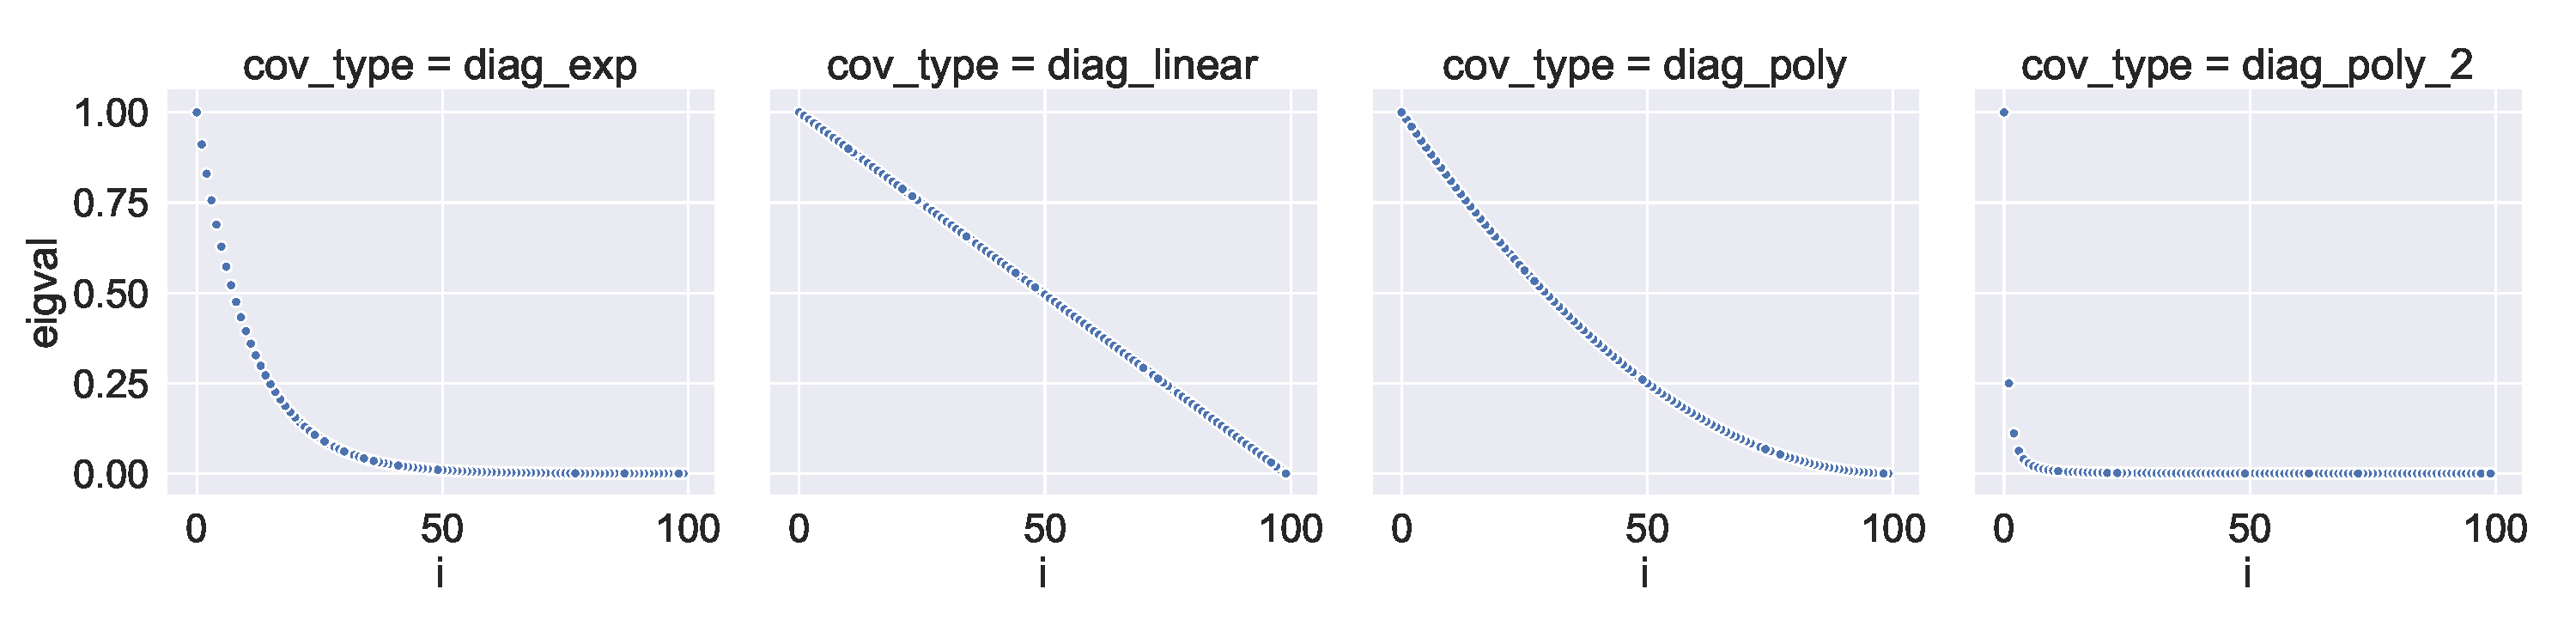
\includegraphics[width=\textwidth]{../continuous_figures/decays.pdf}
  \vspace{-1cm}
  \caption{Scree-plots of $\Sigmab$ for the eigenvalue decays examined
    in our empirical valuations.
    % Here $d=100$ for visualization, whereas
    % our experiments increase $d$ while preserving the ratio $n/d$ and
    % the decay profile,
    % with $\lambda_{\text{max}}(\Sigmab) = 1$ to
    % $\lambda_{\text{min}}(\Sigmab) = 10^{-4}$.
  }
  \label{fig:eig-decays}
\end{figure}


\section{Empirical evaluation of asymptotic consistency}
\label{sec:asymp-conj-details}

% While Theorem~\ref{t:asymptotic} is a result on asymptotic consistency of the
% MSE, the proof (Appendix~\ref{sec:proof-of-t-asymptotic}) follows the standard
% decomposition of MSE in Equation~\ref{eq:mse-derivation} in the process
% establish consistency on the bias and variance terms independently.

% Recall that $\lambda_n=\frac {d-n}{\tr((\Sigmab+\lambda_n\I)^{-1})}$,
% so our surrogate MSE is recovered as
% $\sigma^2\Vc(\Sigmab,n)+\w^{*\top}\Bc(\Sigmab,n)\w^*$.
% % The expressions $\Vc(\Sigmab,n)$ and $\Bc(\Sigmab,n)$ and recover
% % surrogate MSE from Theorem \ref{t:mse} since $\lambda_n=\frac{\tr((\Sigmab+\lambda_n)^{-1})}{d-n}$.
% Lemmas \ref{c:wishart} and \ref{c:projection} provide new insights into classical matrix-variate
% distributions with extensive literature dedicated to them \citep[see,
% e.g.,][]{chikuse1990matrix,cook2011}.
%
%
%

%\section{Empirical evaluation of asymptotic consistency}

% Theorem \ref{t:asymptotic} shows that the surrogate MSE expressions
% derived in Theorem \ref{t:mse} are asymptotically consistent with the
% true MSE for the i.i.d.~design under a class of sub-gaussian data
% distributions.
In this section, we empirically quantify the convergence rates for
the asymptotic result of Theorem~\ref{t:asymptotic}.
% when $\mu$ is a centered multivariate% Gaussian $\Nc(\zero,\Sigmab).$
We focus on the under-determined regime (i.e.,
$n<d$) and separate the evaluation into the bias and
variance terms, following the MSE decomposition given
in \eqref{eq:mse-derivation}. Consider  $\X = \Z\Sigmab^{1/2} $, where the entries of $\Z$ are
i.i.d. standard Gaussian, and define:\vspace{-1mm}
\begin{enumerate}
  \item Variance discrepancy:\quad
    $\big|\frac{\E[\tr((\X^\top\X)^\dagger)]}{\Vc(\Sigmab,n)}-1\big|$ where
    $\Vc(\Sigmab,n)=\frac{1-\alpha_n}{\lambda_n}$.
  \item Bias discrepancy:\quad
     $\sup_{\w\in\R^d\backslash\{\zero\}}\big|\frac{\w^\top\E[\I-\X^\dagger\X]\w}
     {\w^\top\Bc(\Sigmab,n)\w} - 1\big|$
    where $\Bc(\Sigmab,n) = \lambda_n(\Sigmab+\lambda_n\I)^{-1}$.
  \end{enumerate}\vspace{-1mm}
   Recall that $\lambda_n=\frac {d-n}{\tr((\Sigmab+\lambda_n\I)^{-1})}$,
so our surrogate MSE can be written as
$\Mc=\sigma^2\Vc(\Sigmab,n)+\w^{*\top}\Bc(\Sigmab,n)\w^*$, and when both
discrepancies are bounded by $\epsilon$, then $(1-2\epsilon)\Mc\leq\MSE{\X^\dagger\y}\leq (1+2\epsilon)\Mc$.
In our experiments, we consider four standard eigenvalue decay profiles
for $\Sigmab$, including polynomial and exponential decay (see
 \Cref{fig:eig-decays} and \Cref{sec:eig-decay-details}).
\begin{figure} %[ht]
  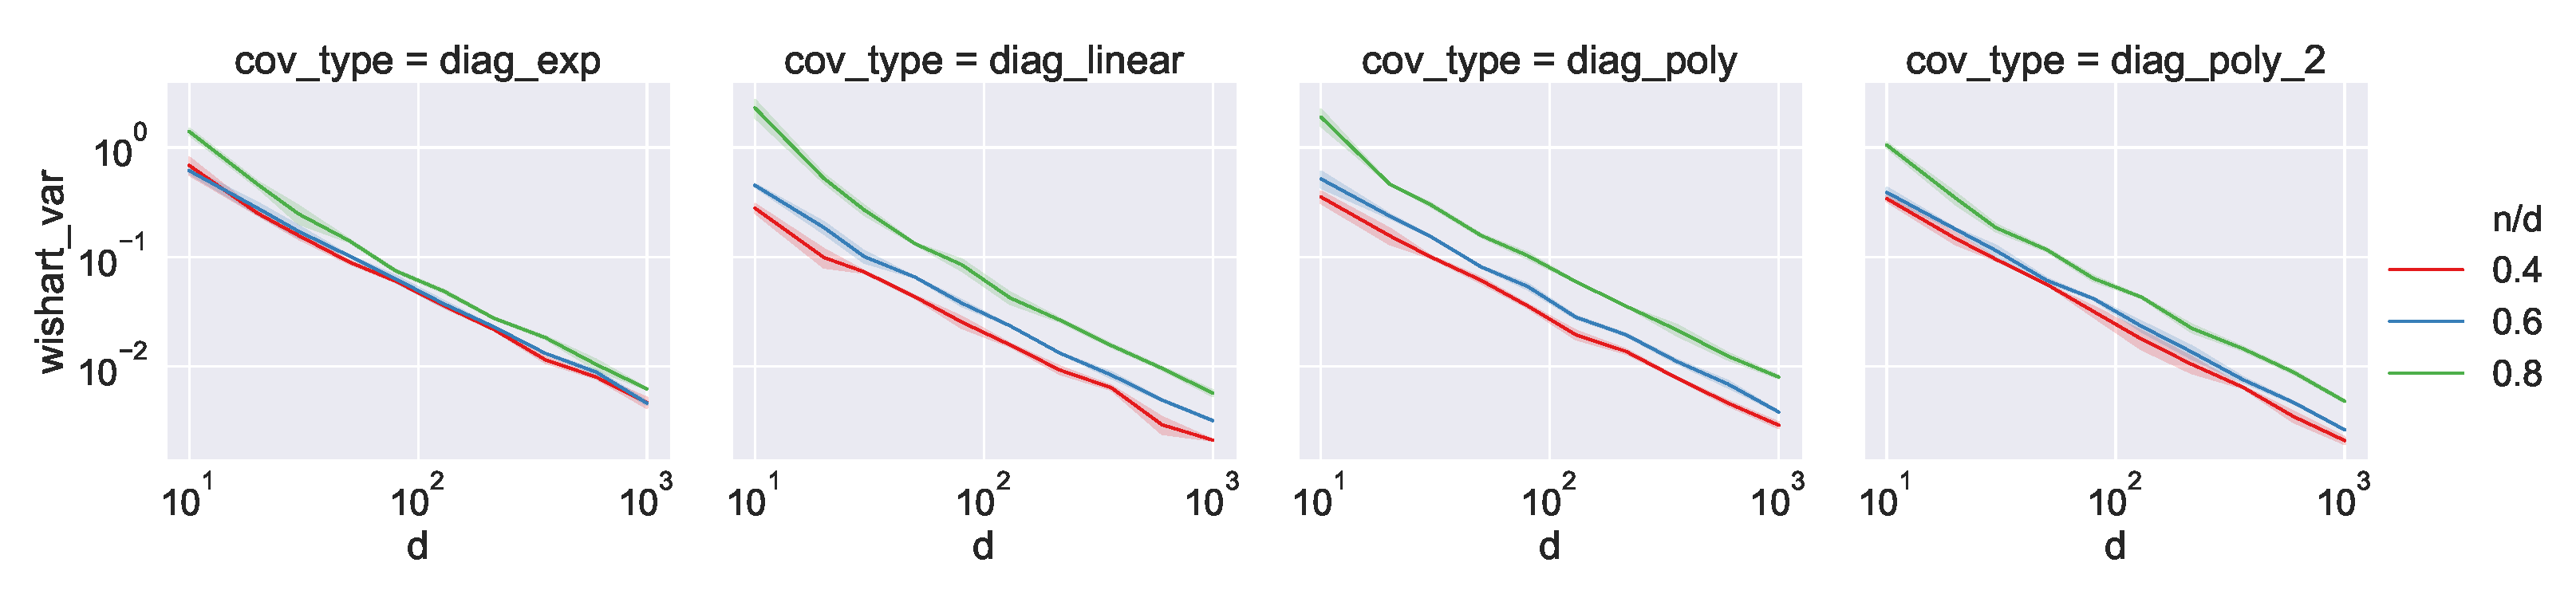
\includegraphics[width=\textwidth]{../continuous_figures/wishart_var.pdf}
  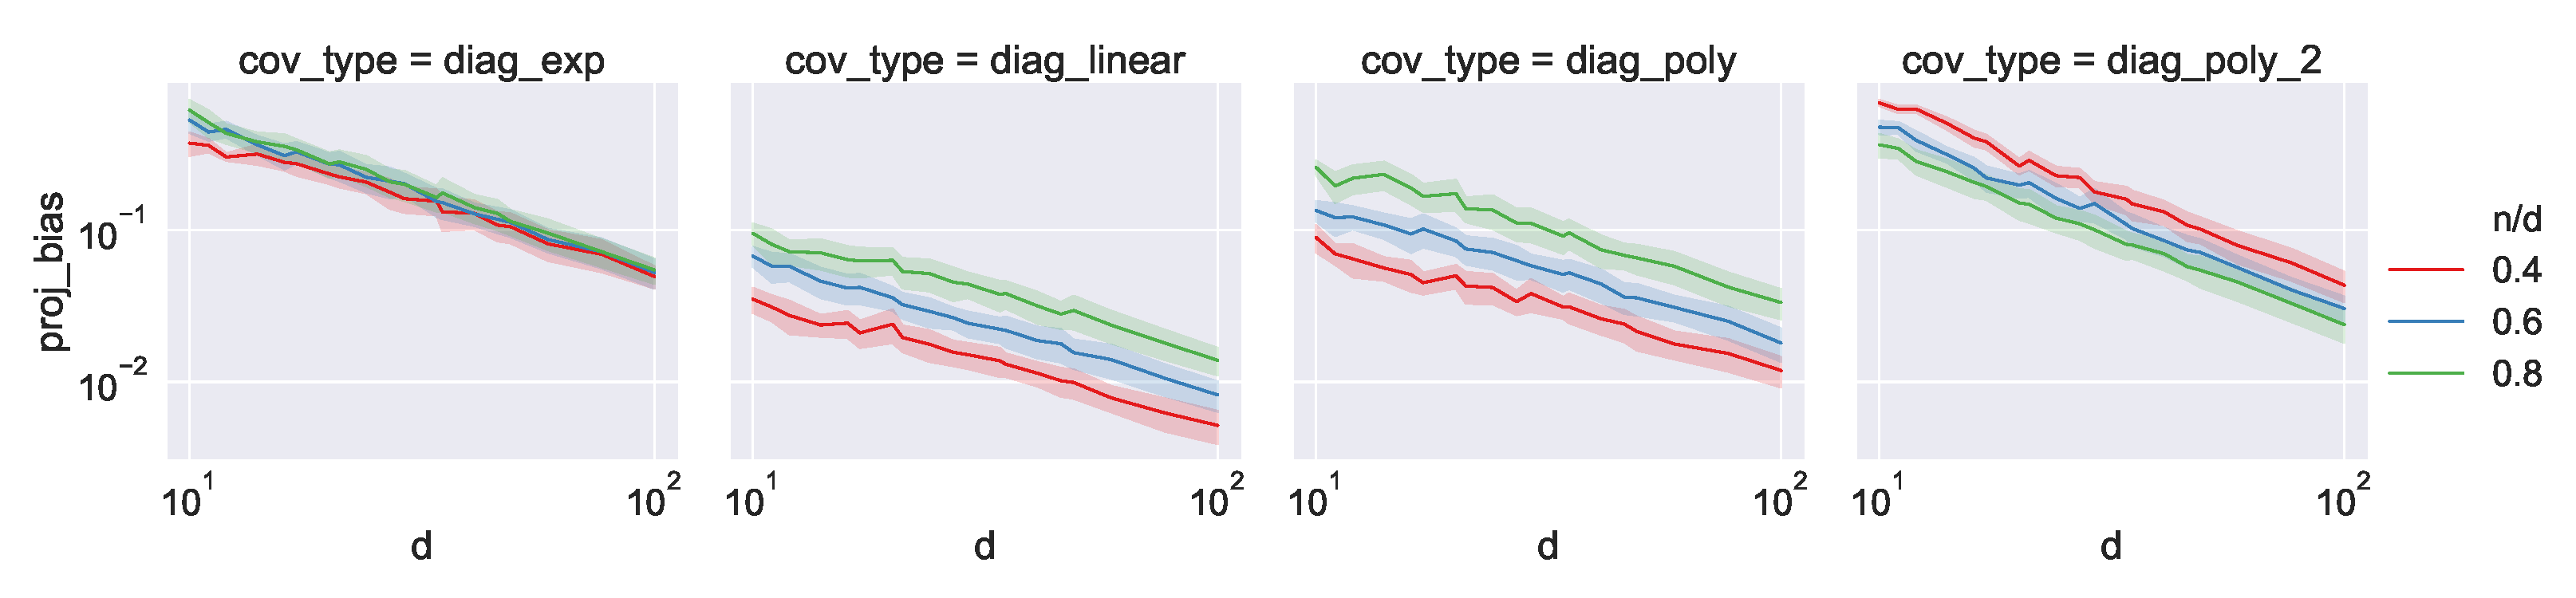
\includegraphics[width=\textwidth]{../continuous_figures/proj_bias.pdf}
  \vspace{-.8cm}
  \caption{
    Empirical verification of the asymptotic consistency of surrogate MSE.
    We show the discrepancies for the variance (top) and bias
    (bottom),  with bootstrapped $95\%$ confidence intervals, as $d$
    increases and $n/d$ is fixed. We observe
     $O(1/d)$ decay (linear with slope $-1$ on a log-log plot).
  }
  \label{f:conj-wishart}
\end{figure}

Figure~\ref{f:conj-wishart} (top) plots the variance discrepancy (with
$\E[\tr((\X^\top\X)^\dagger)]$ estimated via Monte Carlo
sampling and bootstrapped confidence intervals) as $d$ increases from $10$ to
$1000$, across a range of aspect ratios $n/d$. In all cases, we observe that
the discrepancy decays to zero at a rate of $O(1/d)$.
Figure~\ref{f:conj-wishart} (bottom) plots the bias discrepancy, with the same
rate of decay observed throughout.  Note that the range of $d$ is smaller than
in Figure \ref{f:conj-wishart} (top) because the large number of Monte Carlo
samples (up to two million) required for this experiment made the computations
much more expensive (more details in Appendix \ref{a:empirical}). Based on the
above empirical results, we conclude with a conjecture.
\begin{conjecture}
  \label{c:1-over-d-rate}
  When $\mu$ is a centered multivariate Gaussian and its covariance
  has a constant condition
  number, then, for $n/d$ fixed, the surrogate MSE satisfies:
  $\big|\frac{\textnormal{MSE}[\X^\dagger\y]}{\Mc}-1\big|= O(1/d)$.
\end{conjecture}

% The results of empirically validating \Cref{c:wishart} are illustrated in
% Figure~\ref{f:conj-wishart} (top), where we performed Monte Carlo estimation of
% $\E\big[\tr((\X^\top\X)^\dagger)\big]$ and plot
% $\big|\E[\tr((\X^\top\X)^\dagger)]\,\Vc(\Sigmab,n)^{-1} -1\big|$ as $d$ increases from
% $10$ to $1000$, across a range of aspect ratios $n/d$ and eigenvalue decay
% profiles for $\Sigmab$.
% We observe that on log-log axes all of the plots are
% decreasing with a linear $-1$ slope, consistent with the $O(1/d)$ rate
% predicted by \Cref{c:wishart}. \Cref{c:projection} is handled similarly, by
% sampling $\X\sim\mu^n$ where $\mu=\Nc(\zero,\Sigmab )$ to obtain a Monte Carlo
% estimate of $\E[\I-\X^\dagger\X]$.

% Figure~\ref{f:conj-wishart} (bottom) shows how \eqref{eq:projection} decays as
% we hold the aspect ratio $n/d$ fixed and increase $d$ between $10$ and $100$
% across the listed eigenvalue decay profiles and aspect ratios. Again, we
% observe on log-log axes a linear decay with slope $-1$ consistent with the
% $O(1/d)$ rate posed by \Cref{c:projection}. Note that the range of $d$ is
% smaller than in Figure \ref{f:conj-wishart} (top) because the large number of
% Monte Carlo samples (up to two million) required for this experiment made the
% computations much more expensive.



